\chapter{Introduction}
\label{chapter_introduction}

% De Intro en Synthese hoeven van mij geen lange verhalen te zijn, maar moeten het werk dat in % de hoofdstukken staat in de wetenschappelijke context plaatsen. Hier moeten dus de praktische % vragen worden gesteld die hebben geleid tot babette, pirouette en rakette /razzo (Intro) en 
% wat we hier dan mee kunnen (Synthese). Je kunt in de Intro ook wat meer kwijt over hoe BEAST2 % nu eigenlijk werkt, wetenschappelijk gezien, dwz wat zijn species tree priors, wat is de
%  posterior, wat zijn subtitutiemodellen en klokmodellen. Je kunt ook aangeven welke opties in 
% BEAST2 nog niet zijn geimplementeerd (en waarom), daarbij in wat meer detail aangevend wat 
% die opties inhouden (bijv. partities, *BEAST).

% Vragen: hoe juist kunnen we fylogenieen construeren?

% Diversiteit
% Soortvorming
% Verwantschap
% Fylogenie
% DNA
% Bayesiaanse analyse
% Priors









%% Start the actual chapter on a new page.
\newpage

\noindent 
\dropcap{S}{peciation} is the process that creates new species,
connecting all of life to one shared common ancestor. It is a process
that has resulted in the millions of species on Earth nowadays, 
as well as in the many species that have gone extinct. 
Some speciation events happened earlier than others,
from hundreds of millions of years ago (so-called 'long-enduring species',
or, informally, 'living fossil') 
to more recent ones. See figure \ref{fig:long_enduring_and_young_species} 
shows an example of each.

\begin{figure}[H]
  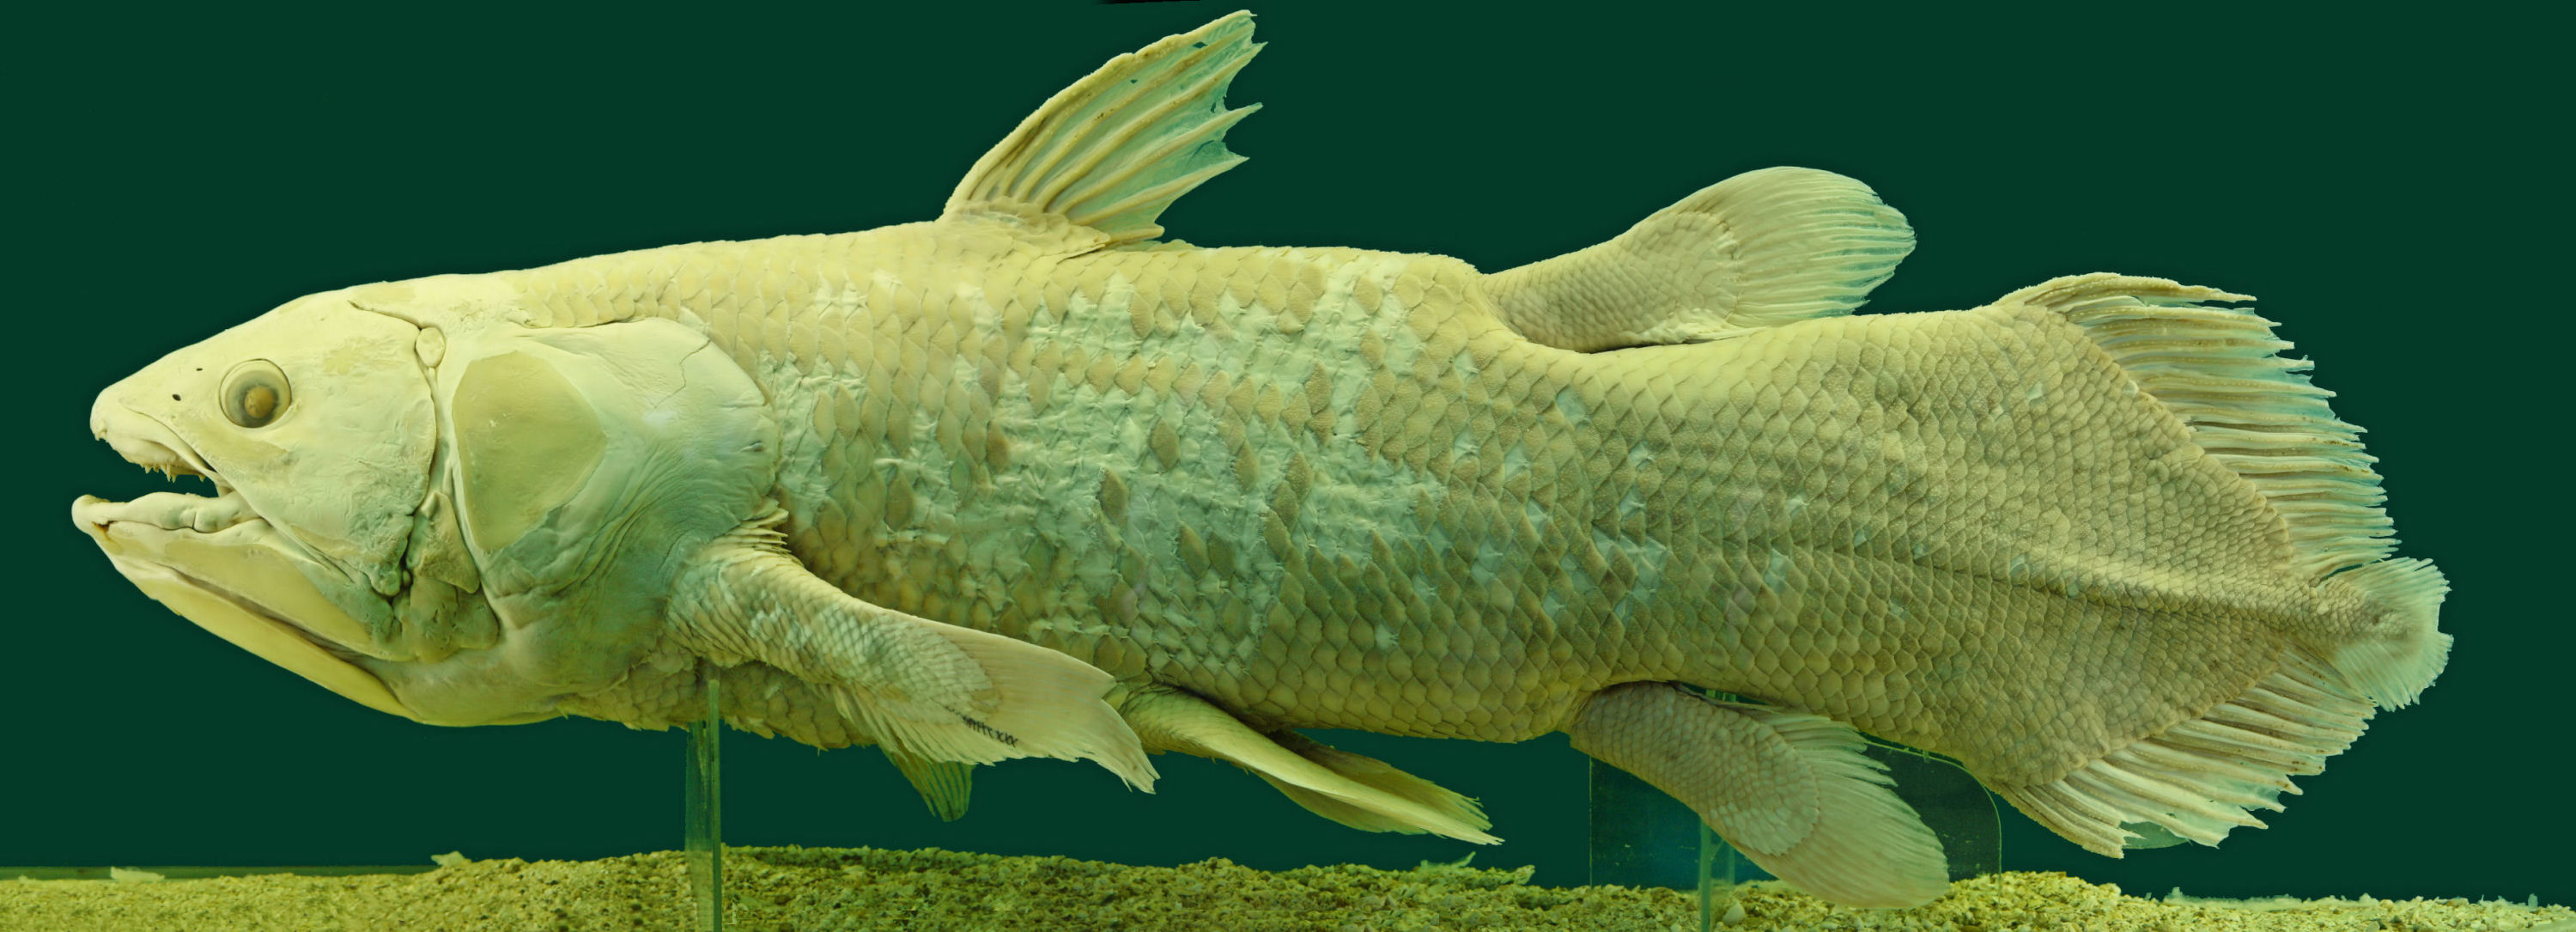
\includegraphics[width=0.5\textwidth]{latimeria_chalumnae.jpg}
  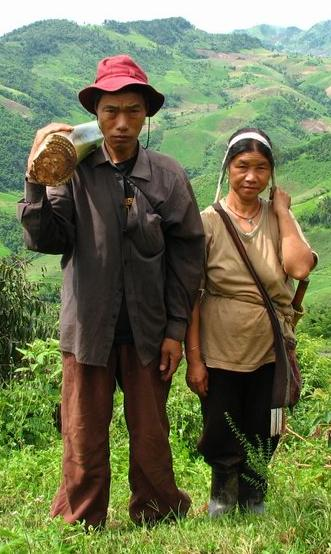
\includegraphics[width=0.2\textwidth]{homo_sapiens.jpg}
  \caption{
    An long-enduring species (left) and a young species (right).
    The species at the left is a preserved specimen of \textit{Latimeria chalumnae}, 
    estimated to exist for hundreds of millions of year.
    The species at the right is the \textit{Homo sapiens}, 
    existing for around a third of a million years.
  }
  \label{fig:long_enduring_and_young_species}
\end{figure}


A first very basic question within the field of biology,
is to ask which species are closest related to
one another. If you think that's an easy question, try to apply it, 
for example, on the 8 crocodilian pictures in figure \ref{fig:crocodialians}.
You may come up with one or more pairs of hypothesized closest-related species,
but you will probably get stuck on which ancestors of these pairs
are most closely related. Note that doing the other way around, to use
morphology to classify species, is tricky: how to decide when the morphology 
between two specimens is different enough to classify these as two species?

\begin{figure}[H]
  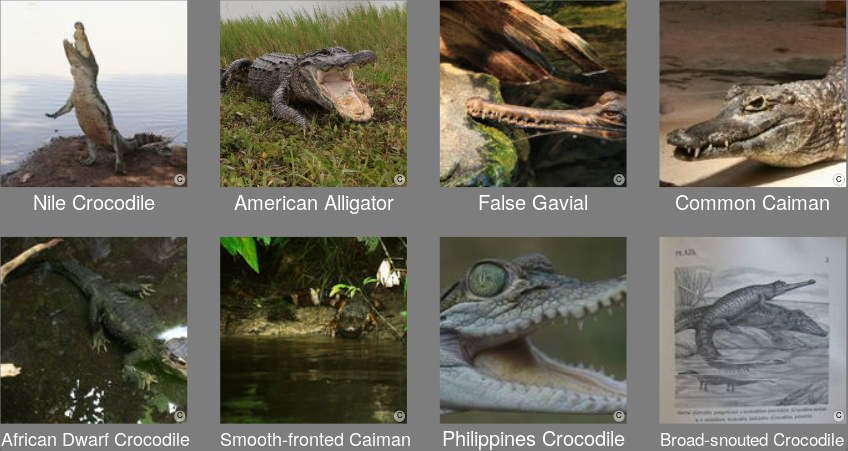
\includegraphics[width=1.0\textwidth]{crocodilians.png}
  \caption{
    Eight members of the order of crocodilians
  }
  \label{fig:crocodialians}
\end{figure}

The second very basic biological question, is to 
ask \emph{when} these speciation events took place.
This question cannot be answered based on morphologies of the present-day
species alone, because morphology is a complex trait, and the pace at
which morphology changes in time is unknown or unpredictable.

This second question can be answered by
using a classical approach, 
by using the morphology of fossils.
This approach can only be used if the species \emph{can} fossilize,
and those fossils are found in multiple points in time.
Even if this is the case, there are caveats. Using morphology on
extinct species is even trickier, as species change their appearance in time.
Also an imaginary time machine would not help us out:
we could try to determine the number of species in each timepoint,
but that would only work if we could confidently define what a
species is. We cannot, because speciation is usually a gradual process.

This second question can also be answered 
using a modern approach, 
by using the DNA sequences of extant species,
as shown, for example, in figure \ref{fig:alignment}.
Because DNA is inherited from parent to offspring
and changes through times, it carries each species' 
evolutionary histories within it.
The point in time when a species speciates is
marked by the two daughter species having seperate mutations
from that moment on.
Due to this, we can easily find closest related species 
by measuring the similarity in DNA sequences.
If we know how frequent mutations occur, we can already
do a rough estimation of when the speciation event took place.
In reality, DNA sequences of different species 
varies in length, due to insertions and deletions in genetic sequences,
but in the simulation studies in this thesis, we will ignore this.

\begin{figure}[H]
  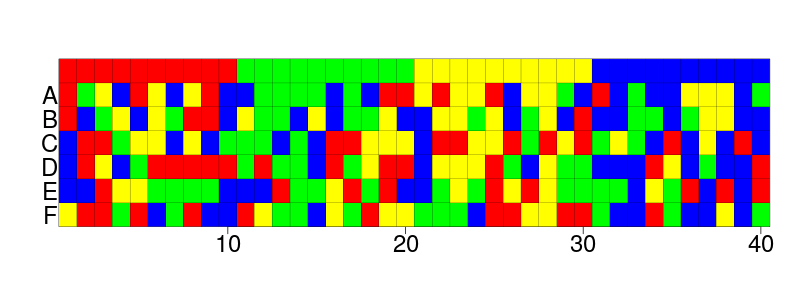
\includegraphics[width=0.8\textwidth]{alignment_40_with_root.png}
  \caption{
    A 40-nucleotide DNA alignment of six hypothetical species. The species
    are named A to and including F. 
    The four colors denote the four different nucleotides,
    in which the red color resembles adenine, yellow depicts cytosine, 
    green is for guanine, and blue resembles thymine. The top
    row shows the (artificial) root sequence, which is usually unknown. 
  }
  \label{fig:alignment}
\end{figure}

Speciation at the species level simplifies a species to a horizontal 
line (also called a 'branch') in a phylogeny, answering
basic questions like 'Which species lived when?', 'When did a speciation 
event take place?' (depicted by the vertical lines)
and 'Who is the ancestor of which species?'. 
Figure \ref{fig:phylogeny} shows an example phylogeny:

\begin{figure}[H]
  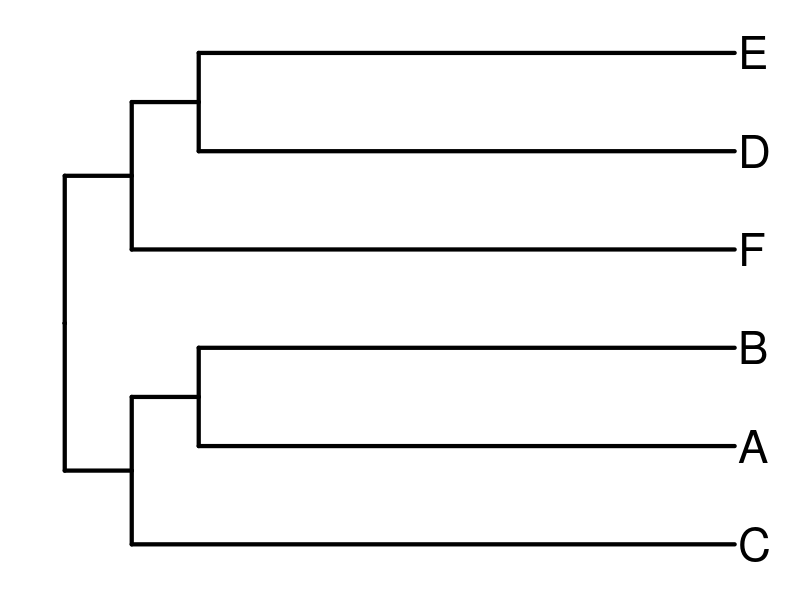
\includegraphics[width=0.4\textwidth]{phylogeny.png}
  \caption{
    A phylogeny with six species
  }
  \label{fig:phylogeny}
\end{figure}

Figure \ref{fig:phylogeny} shows a phylogeny (also called 'phylogenetic tree', 
or simply 'tree') with six hypothetical species and their evolutionary 
relationships. Going from left to right, we travel through time from 
the past to the present. 
The leftmost vertical line indicates the first speciation event, 
which gave rise to the first two ancestral species. 
This first split in the tree is called the crown,
the moment in time this occurred is called the crown age.

Each of these ancestral species gives rise to its own evolutionary history,
resulting in a tree with two clades: the ABC and the DEF clades.
Sure, we could equally well have started the phylogeny 
with one ancestral species at the utmost left,
going further back in time from the crown age to, what is called, the stem age,
but in the context of this thesis, we do not.

It is impossible to go out in the field and measure a phylogy, 
as they depict which species lived when \emph{in the past}. 



The main question of this thesis is: how well can we construct a
phylogeny from an alignment? What is the error we
make when we construct a 'tree without birds'?


Figure \ref{fig:alignment} shows an alignment of our six hypothetical species
that we actually could have found in nature. From this alignment, we
can \emph{infer} a phylogeny, which basically means 'best guess following a 
rational procedure'. There are multiple ways to infer a phylogeny, for
example, using maximum likelihood or Bayesian inference. In this thesis, 
I focus on the latter.

With Bayesian inference, we use an alignment and our model assumptions to infer 
a posterior (more 
precise: 'a joint posterior distribution of phylogenies and model parameters').
We do so, by first creating a random phylogeny. Using a likelihood equation,
we can calculate how likeli it  
For that, we use a Markov Chain Monte Carlo algorithm, which is n 


A posterior contains multiple inferred phylogenies, in which the more likely
ones are present more often. This distribution of phylogenies shows the
(un)certainty of the inference. Figure \ref{fig:densitree} shows the
posterior phylogenies we obtain from our alignment:

\begin{figure}[H]
  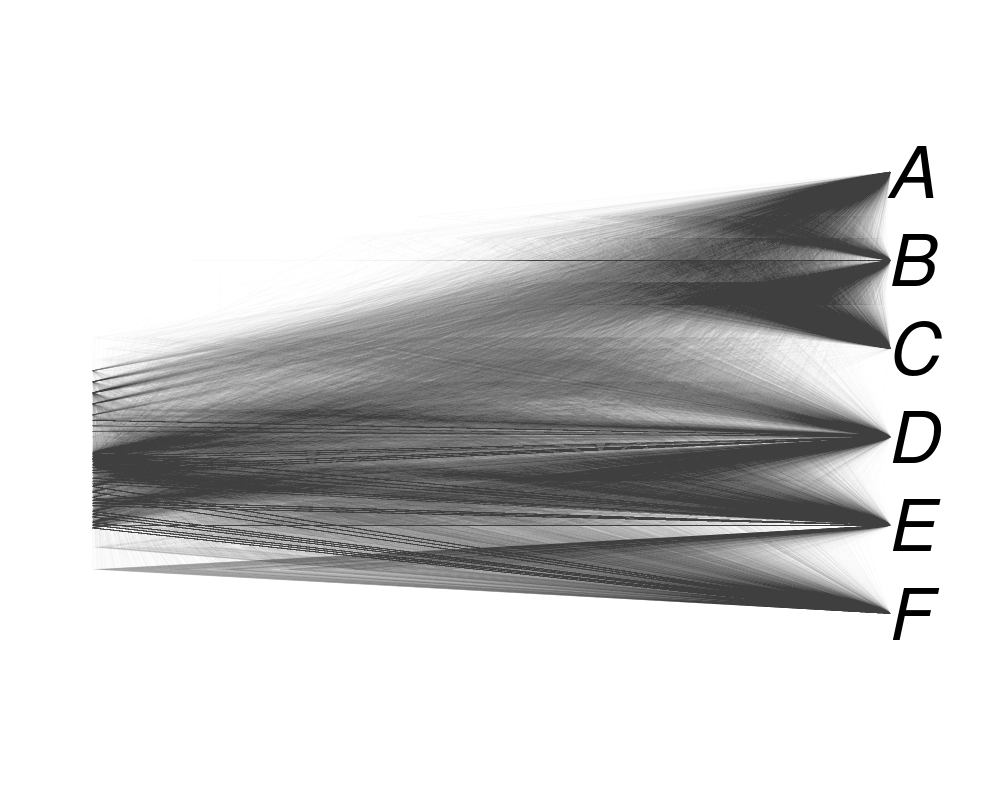
\includegraphics[width=0.8\textwidth]{densitree_40.png}
  \caption{
    The posterior phylogenies of the six species, 
    from a DNA alignment of 40 nucleotides
  }
  \label{fig:densitree}
\end{figure}

Figure \ref{fig:densitree} shows a high degree of uncertainty, as the
inferred phylogenies vary widely in shape. The inference only
weakly distinguishes between the ABC and DEF clades. 

The inference described so far is unsatisfactory, as we can only draw 
weak conclusions. We can improve the inference by using a longer DNA sequence 
or by picking a better inference model. In a simulation study, we can
easily increase the number of nucleotides, 
figure \ref{fig:densitree_again} shows the
posterior phylogenies we obtain from our longer alignment:

\begin{figure}[H]
  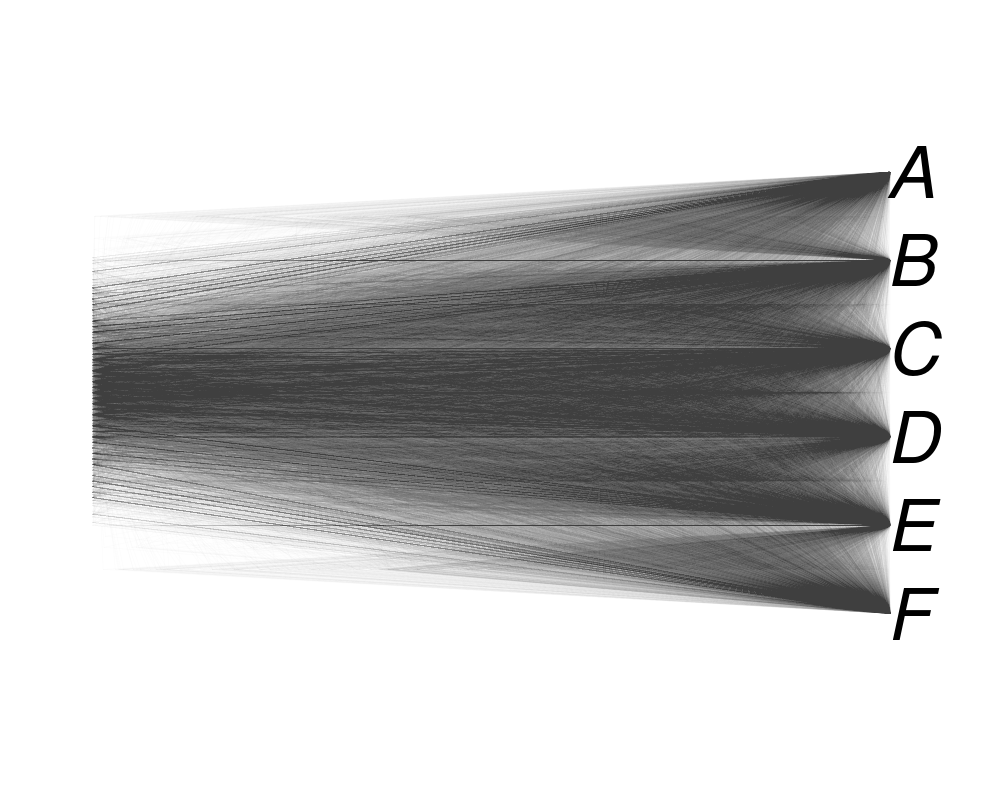
\includegraphics[width=0.8\textwidth]{densitree_400.png}
  \caption{
    The posterior phylogenies of the six species,
    from a DNA alignment of 400 nucleotides
  }
  \label{fig:densitree_again}
\end{figure}

Figure \ref{fig:densitree_again} shows that in this example,
with more information, we can only show our uncertainty more clearly. 

Another way to improve our inference is using a better inference model.
An inference model embodies our assumptions on how we think evolution
works, and consists of (1) how nucleotides mutate to others (also
called 'the site model'), (2) how often mutations occur (also 
called 'the clock model'), and (3) how speciation works (also 
called 'the tree prior' or 'the speciation model'). 
Theory predicts that usually the inference model becomes less important
if there is more information in an alignment. The example shows here,
however, shows one of the exceptions.

Ideally, we pick an inference model identical to the actual way things 
work (or: 'the true model'), be it in nature
or \textit{in silico}. In practice, the true model that nature uses is unknown.
Due to this, scientists came up with many models to explain the 
DNA (RNA, protein, morpholical and fossil) data best.

In a theoretical study, when can simply pick how nature works; that is,
how it is simulated. Theoretical studies are useful, as these explore
how well we will ever be able to explain nature. To do so, a 'true' 
speciation model is picked to generate 'true' phylogenies. 
From these phylogenies, a 'true' site model and clock model are used to
simulate a 'true' alignment. From that 'true' alignment, which is the
data we can gather from nature, we can then see how close our inferred
phylogenies are to the 'true' phylogeny.

\begin{figure}[H]
  \centering
  \subfloat[True tree] {
    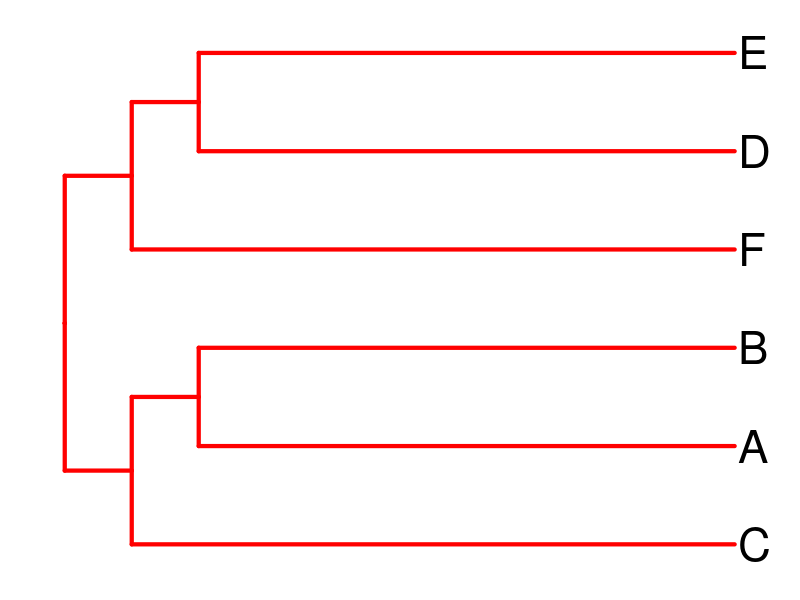
\includegraphics[width=0.3\textwidth]{true_tree.png}
  }
  \subfloat[Twin tree] {
    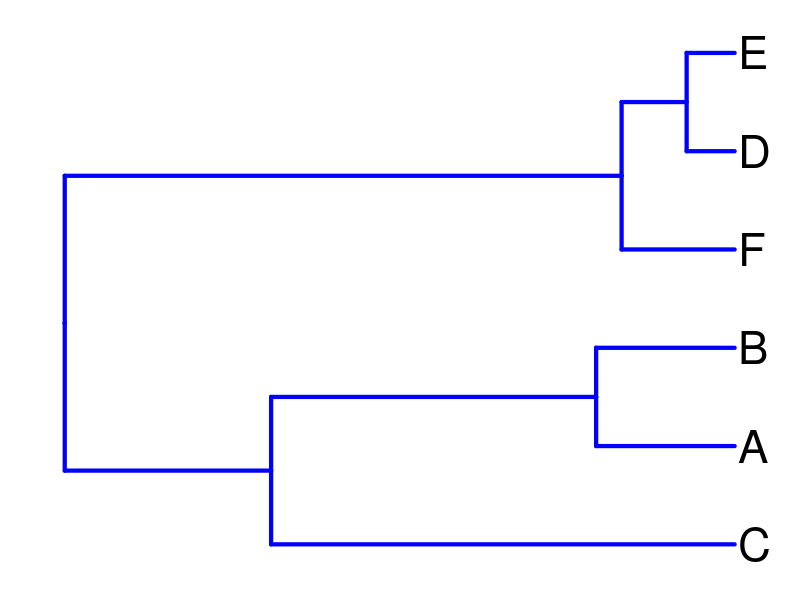
\includegraphics[width=0.3\textwidth]{twin_tree.png}
  } 
  \subfloat[Combined nLTT] {
    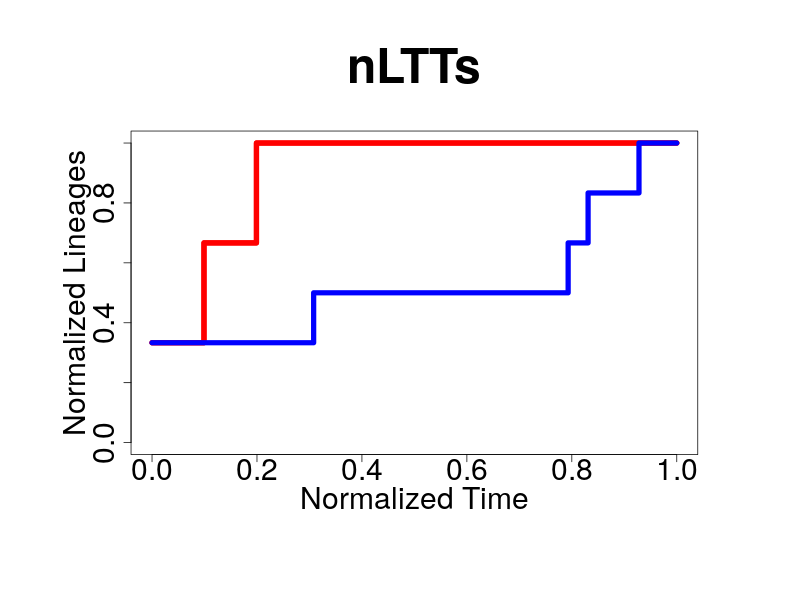
\includegraphics[width=0.4\textwidth]{nltt.png}
  }
  \caption{
    nLTTs
  }
  \label{fig:nltts}
\end{figure}

There are many ways to quantify how similar two phylogenies are. 
The normalized lineages-through-time (nLTT) statistic (\cite{janzen2015approximate}) simplifies
a phylogeny to a number of lineages (the number of branches) in time.
Both number of lineages and time are normalized to have a maximum of one,
which allows us to compare two trees of any number of tips of any crown age.
The difference between two phylogenies is simply the surface between the
two phylogenies' nLTT plots. If two phylogenies are identical in 
normalized shape, the nLTT difference between them in zero, else the
value will be higher, with a maximum of one. Because the value of the 
nLTT increases with increasing difference between the trees, the nLTT statistic
is a measure of difference, or error. 

In this thesis, I quantify the errors we make in our phylogenetic inference:

\begin{itemize}
	\item In chapter 2, I show an R package I developed to do Bayesian
    inference from the command-line
	\item In chapter 3, me and Giovanni Laudanno describe an R package we 
    developed to quantify the error we make in phylogenetic inference
	\item In chapter 4, Giovanni Laudanno and I quantify the error we make 
    in phylogenetic trees when speciation can co-occur
	\item In chapter 5, I quantify the error we make 
    in phylogenetic trees when speciation takes time
	\item In chapter 6, I show which conclusions can be drawn from these chapters
\end{itemize}

\references{dissertation}


\subsection{Photo attribution}

Figure \ref{fig:long_enduring_and_young_species},
the left image,
\href{https://en.wikipedia.org/wiki/File:Latimeria_Chalumnae_-_Coelacanth_-_NHMW.jpg}{Preserved specimen of chalumnae}
by Alberto Fernandez Fernandez
is licensed under \href{https://creativecommons.org/licenses/by-sa/3.0/deed.en}{CC BY-SA 3.0}.
the image at the right,
\href{https://commons.wikimedia.org/wiki/File:Akha_cropped_hires.JPG}{Akha couple in northern Thailand}
by Weltenbummler84
is licensed under \href{https://creativecommons.org/licenses/by-sa/2.0/de/deed.en}{CC BY-SA 2.0 DE}.

For figure \ref{fig:crocodialians},
the selection of these eight images was done by 
\href{https://www.onezoom.org/life.html/@Crocodylia=195672\#x1602,y148,w4.1516}{OneZoom}.
These images, from top-left to bottom-row, row-first:
% 1
\href{http://media.eol.org/content/2018/04/11/13/61270_orig.jpg}{Nile Crocodile}
by Marco Schmidt
is licensed under \href{http://creativecommons.org/licenses/by-sa/3.0}{CC-BY-SA 3.0}.
% 2
\href{https://www.flickr.com/photos/nasakennedy/14159295507}{American Alligator}
by NASA Kennedy.
% 3
\href{http://media.eol.org/content/2014/10/06/10/58393_orig.jpg}{False Gavial}
by Yinan Chen
is marked as being in the public domain.
% 4
\href{http://media.eol.org/content/2012/06/13/05/87714_orig.jpg}{Common Caiman}
by Michael Wolf
is licensed under \href{http://creativecommons.org/licenses/by/2.5}{CC-BY 2.5}.
% 5
\href{http://media.eol.org/content/2013/06/11/03/12146_orig.jpg}{African Dwarf Crocodile}
by Staycoolandbegood
is marked as being in the public domain.
% 6
\href{http://media.eol.org/content/2013/11/25/21/58484_orig.jpg}{Smooth-fronted Caiman}
by Whaldener Endo
is licensed under \href{http://creativecommons.org/licenses/by-sa/4.0}{CC-BY-SA 4.0}
% 7
\href{http://media.eol.org/content/2013/06/11/03/06619_orig.jpg}{Phillipines Crocodile}
by Vanderploeg
is marked as being in the public domain.
% 8
\href{http://media.eol.org/content/2014/10/06/16/93746_orig.jpg}{Board-snouted Crocodile}
by Hadonos
is Marked as being in the public domain.
